\documentclass[border=2]{standalone}
\usepackage{tikz}

\usetikzlibrary{arrows, arrows.meta, positioning}

\tikzset{    
    disk/.style={ thick },
    traj/.style={ thin, dashed, -Latex },
    point/.style={ color=black, circle, scale=0.3, fill },
    partition/.style={ right, scale=0.75 },
    label/.style={ scale=0.5, black, below = 0.5mm },
    time/.style={ scale=1, above right }
}

\def\xMin{0}
\def\xMax{8}
\def\yMin{0}
\def\yMax{8}
\def\xWidth{1}
\def\oPacity{0.75}
\def\ySlant{0.5}
\def\xSlant{-1.0}
\def\z{80}
\def\speed{0.20}
\def\R{0.10}

\newcommand{\drawBlueFrame}[5]{
    \fill[blue, opacity=0.05] (#1*\xWidth-#5,#2*\xWidth-#5) rectangle (#3*\xWidth+#5,#4*\xWidth+#5);
    \draw[blue, opacity=0.05] (#1*\xWidth-#5,#2*\xWidth-#5) rectangle (#3*\xWidth+#5,#4*\xWidth+#5);
}

\newcommand{\drawWhiteFrame}[5]{
    \fill[white, opacity=0.5] (#1*\xWidth-#5,#2*\xWidth-#5) rectangle (#3*\xWidth+#5,#4*\xWidth+#5);
    \draw[black, dashed, opacity=0.5] (#1*\xWidth-#5,#2*\xWidth-#5) rectangle (#3*\xWidth+#5,#4*\xWidth+#5);
}

\newcommand{\drawFrame}[4]{
        \drawBlueFrame{#1}{#2}{#3}{#4}{0*\speed};
        \drawWhiteFrame{#1}{#2}{#3}{#4}{-1*\speed};
}

\newcommand{\drawGrid}{
    \draw[dashed, fill=white,fill opacity=\oPacity] (\xMin,\yMin) rectangle (\xMax,\yMax);
    \draw[dashed] (0,4) -- (8,4);
    \draw[dashed] (0,6) -- (8,6);
    \draw[dashed] (0,2) -- (4,2);
    \draw[dashed] (0,1) -- (2,1);
    \draw[dashed] (0,1) -- (2,1);
    \draw[dashed] (2,7) -- (4,7);
    
    \draw[dashed] (4,0) -- (4,8);
    \draw[dashed] (2,0) -- (2,8);
    \draw[dashed] (6,4) -- (6,8);
    \draw[dashed] (1,0) -- (1,2);
    \draw[dashed] (3,6) -- (3,8);
    
    \draw[step=\xWidth, very thin, black!15] (\xMin,\yMin) grid (\xMax,\yMax);
}

\newcommand{\drawAFlocks}[0]{
    \draw [fill=olive] (A1) circle (\R) ;
    \draw [fill=olive] (A2) circle (\R) ;
    \draw [fill=olive] (A3) circle (\R) ;
    \draw [fill=olive] (A4) circle (\R) ;
}
\newcommand{\drawBFlocks}[0]{
    \draw [fill=teal] (B1) circle (\R) ;
    \draw [fill=teal] (B2) circle (\R) ;
    \draw [fill=teal] (B3) circle (\R) ;
    \draw [fill=teal] (B4) circle (\R) ;
}
\newcommand{\drawCFlocks}[0]{
    \draw [fill=magenta] (C1) circle (\R) ;
    \draw [fill=magenta] (C2) circle (\R) ;
    \draw [fill=magenta] (C3) circle (\R) ;
    \draw [fill=magenta] (C4) circle (\R) ;
}

\begin{document}
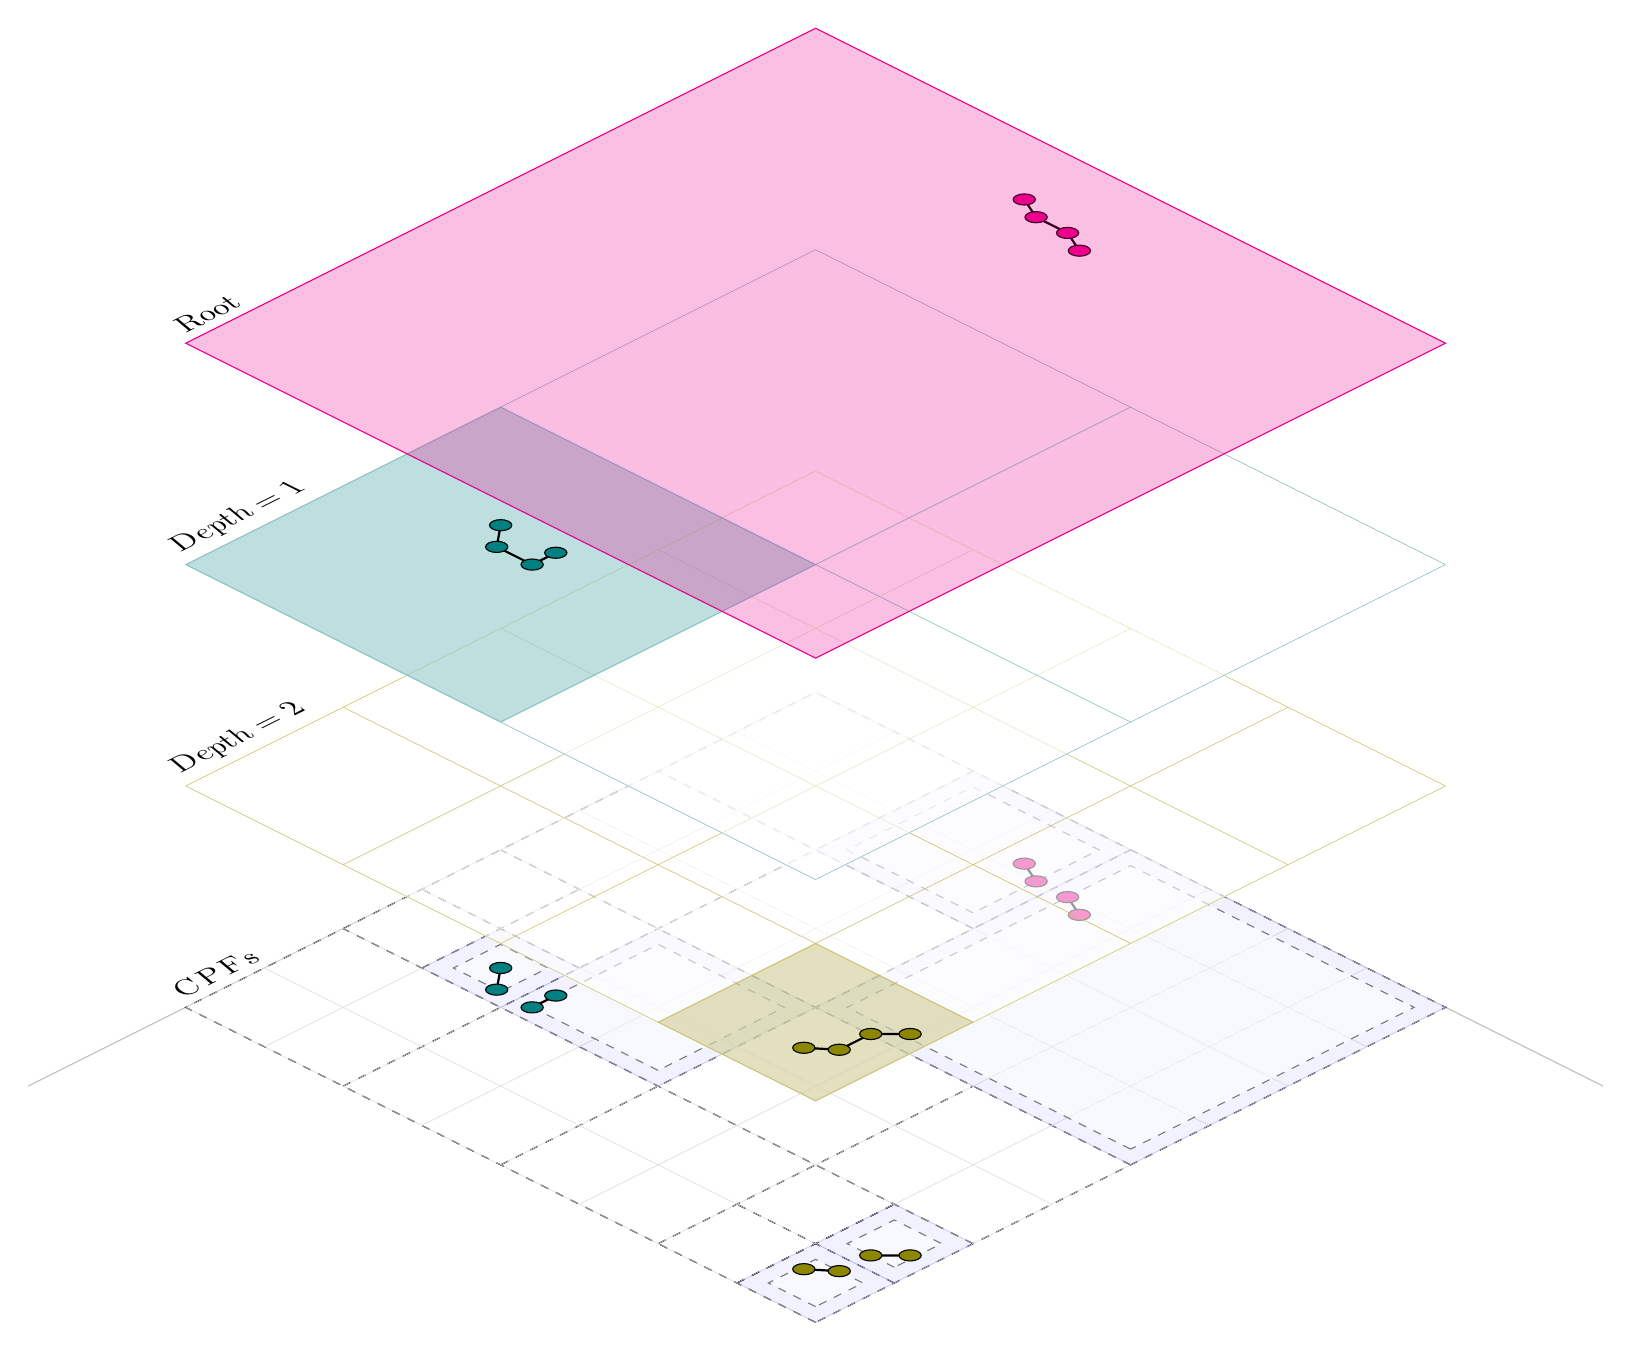
\begin{tikzpicture}    
    \def\t{0};
    \begin{scope}
        [yshift=0*\z, every node/.append style={yslant=\ySlant,xslant=\xSlant},yslant=\ySlant,xslant=\xSlant]
        \coordinate (O) at (\xMax,\yMax);

        \draw[black!25] (O) -- (\xMax,-2);
        \draw[black!25] (O) -- (-2,\yMax);
        
        \coordinate (T) at (\xMin, \xMax);
        \node[time] at (T) {$CPFs$};

        \coordinate (A1) at (0.60, 0.75);
        \coordinate (A2) at (0.80, 0.50);
        \coordinate (A3) at (1.20, 0.50);
        \coordinate (A4) at (1.45, 0.25);

        \coordinate (B1) at (2.50, 6.50);
        \coordinate (B2) at (2.20, 6.25);
        \coordinate (B3) at (2.20, 5.80);
        \coordinate (B4) at (2.50, 5.80);

        \coordinate (C1) at (7.15, 4.50);
        \coordinate (C2) at (7.00, 4.20);
        \coordinate (C3) at (7.00, 3.80);
        \coordinate (C4) at (6.85, 3.50);

        \drawGrid
        \drawFrame{0}{0}{1}{1};
        \drawFrame{1}{0}{2}{1};
        \drawFrame{2}{6}{3}{7};
        \drawFrame{2}{4}{4}{6};
        \drawFrame{4}{0}{8}{4};
        \drawFrame{6}{4}{8}{6};
        \draw[thick] (A1) -- (A2);
        \draw[thick] (A3) -- (A4);
        \drawAFlocks
        \draw[thick] (B1) -- (B2);
        \draw[thick] (B3) -- (B4);
        \drawBFlocks
        \draw[thick] (C1) -- (C2);
        \draw[thick]  (C3) -- (C4);
        \drawCFlocks
    \end{scope}

    \def\t{1};
    \begin{scope}
        [yshift=1*\z, every node/.append style={yslant=\ySlant,xslant=\xSlant},yslant=\ySlant,xslant=\xSlant]

        \coordinate (T) at (\xMin, \xMax);
        \node[time] at (T) {$Depth = 2$};

        \draw[white, fill=white, fill opacity=0.6] (0,0) rectangle (8, 8);
        \draw[olive, fill=olive, opacity=0.25] (0,0) rectangle (2,2);
        \coordinate (A1) at (0.60, 0.75);
        \coordinate (A2) at (0.80, 0.50);
        \coordinate (A3) at (1.20, 0.50);
        \coordinate (A4) at (1.45, 0.25);

        \draw[step=2, very thin, olive!50] (\xMin,\yMin) grid (\xMax,\yMax);
        \draw[thick] (A1) -- (A2) -- (A3) -- (A4);
        \drawAFlocks
    \end{scope}
    
    \def\t{2};
    \begin{scope}
        [yshift=2*\z, every node/.append style={yslant=\ySlant,xslant=\xSlant},yslant=\ySlant,xslant=\xSlant]

        \coordinate (T) at (\xMin, \xMax);
        \node[time] at (T) {$Depth = 1$};

        \draw[white, fill=white, fill opacity=0.6] (0,0) rectangle (8, 8);
        \draw[teal, fill=teal, opacity=0.25] (0,4) rectangle (4,8);
        \coordinate (B1) at (2.50, 6.50);
        \coordinate (B2) at (2.20, 6.25);
        \coordinate (B3) at (2.20, 5.80);
        \coordinate (B4) at (2.50, 5.80);

        \draw[step=4, very thin, teal!50] (\xMin,\yMin) grid (\xMax,\yMax);
        \draw[thick] (B1) -- (B2) -- (B3) -- (B4);
        \drawBFlocks
    \end{scope}

    \def\t{3};
    \begin{scope}
        [yshift=3*\z, every node/.append style={yslant=\ySlant,xslant=\xSlant},yslant=\ySlant,xslant=\xSlant]

        \coordinate (T) at (\xMin, \xMax);
        \node[time] at (T) {$Root$};

        \coordinate (C1) at (7.15, 4.50);
        \coordinate (C2) at (7.00, 4.20);
        \coordinate (C3) at (7.00, 3.80);
        \coordinate (C4) at (6.85, 3.50);
        
        \draw[thick] (C1) -- (C2) -- (C3) -- (C4);
        \drawCFlocks
        \draw[magenta, fill=magenta, fill opacity=0.25] (0,0) rectangle (8,8);
    \end{scope}
    
\end{tikzpicture}
\end{document} 
